\documentclass[compress]{beamer}
\setbeamercolor{normal text}{fg=white}
\setbeamercovered{transparent, still covered={\opaqueness<1->{0}}, again covered={\opaqueness<1->{30}}}
\beamertemplatesolidbackgroundcolor{black}
\usecolortheme[named=white]{structure} 
\usepackage{caption}
\captionsetup{labelformat=empty}
\setbeamertemplate{navigation symbols}{} 
%\usefonttheme{structurebold}
\usepackage{listings}
\usepackage{ulem}
\usepackage[scaled]{helvet}
\renewcommand*\familydefault{\sfdefault} %% Only if the base font of the document is to be sans serif
\usepackage[T1]{fontenc}
\usepackage{setspace}
%\usepackage{beamerthemesplit}
\usepackage{graphics}
\usepackage{hyperref}
\usepackage{graphicx}
\usepackage{verbatim}
\usepackage{amssymb}
\usepackage{wrapfig}
\usefonttheme[onlymath]{serif}
\usepackage{cmbright}

\def\labelitemi{\textemdash}
\setbeamertemplate{frametitle}{
	\begin{centering}
		\vskip15pt
		\insertframetitle
		\par
	\end{centering}
} 
\title[Names]{\\ \vspace{10mm} learning from names}
\author[Sood and Laohaprapanon]{gaurav and suriyan}
  \large
\date[2019]{}
\subject{Paper}
\begin{document}
\newcommand{\multilineR}[1]{\begin{tabular}[b]{@{}r@{}}#1\end{tabular}}
\newcommand{\multilineL}[1]{\begin{tabular}[b]{@{}l@{}}#1\end{tabular}}
\newcommand{\multilineC}[1]{\begin{tabular}[b]{@{}c@{}}#1\end{tabular}}
\newcommand{\indep}{\rotatebox[origin=c]{90}{$\models$}}
\newenvironment{large_enum}{
\Large
\begin{itemize}
  \setlength{\itemsep}{7pt}
  \setlength{\parskip}{0pt}
  \setlength{\parsep}{0pt}
}{\end{itemize}}

\begin{comment}

setwd(paste0(githubdir, "ethnicolr_paper/present/"))
tools::texi2dvi("sequence_of_chars.tex", pdf = TRUE, clean = TRUE)
setwd(basedir)

\end{comment}
  \frame
  {
    \titlepage
  }

\frame{

\Large{Why Learn From Names?}
\pause

\begin{large_enum}
	\item[-]<2>Because sometimes all you have is names
	\item[-]<3->\alert<4>{Media}, most voter lists, \ldots
\end{large_enum}
}

\frame{
	\texttt{WASHINGTON --- Some of \alert<2>{Robert S. Mueller III's} investigators have told associates that Attorney General \alert<2>{William P. Barr} failed to adequately portray the findings of their inquiry and that they were more troubling for President Trump than Mr. Barr indicated, according to government officials and others familiar with their simmering frustrations.}\\ 

	\vspace{20mm}
	\small{Source: The New York Times}
}

\frame{
\Large{Why Learn From Names?}
\begin{large_enum}
	\item[-]<0>Because sometimes all you have are names
	\item[-]<0>Media, most voter lists, \ldots
	\item[-]<2-6>But you want to:
		\begin{itemize}
			\item[-]<3->Highlight biases
			\item[-]<4->Fight biases
			\item[-]<5->Prevent biases (Regress Out)
			\item[-]<6->Personalize
		\end{itemize}
	\item[-]<7-11>Concretely:
		\begin{itemize}
			\item[-]<8->Biases in media coverage: who is (covered) cited as a source?, \ldots
			\item[-]<9->Fairness in lending
			\item[-]<10->Political accountability: whose emails are read?, \ldots 
			\item[-]<11->Personalization---recommending same race doctor (Alsan et al. 2018)
		\end{itemize}
	\end{large_enum}
}

\frame{

\Large{Why \only<2->{\alert{Not}} Learn From Names?}
\pause

\begin{large_enum}
	\item[-]<3> Instrument for Discrimination
	\item[-]<4> But that risk exists for credit risk scoring too.
	\item[-]<5> To enable predatory lending
	\item[-]<6> But still a concern \ldots
\end{large_enum}
}

\frame{

\Large{But if we were to learn from names, how would we?}
\pause

\begin{large_enum}
	\item[-]<2>$p\;(\text{ethnicity\;}|\;\text{name})$?
	\item[-]<3> Classify to the majority class
	\item[-]<4> Makes the least mistakes---Bayes Optimal Error
	\item[-]<5-6> Census Last Name Dataset
		\begin{itemize}
			\item[-]<6->Split by race for 1,000 most common last names
		\end{itemize}
	\end{large_enum}
}

{
\setbeamercolor{background canvas}{bg=white}
\begin{frame}
	\center{{\scalebox{0.6}{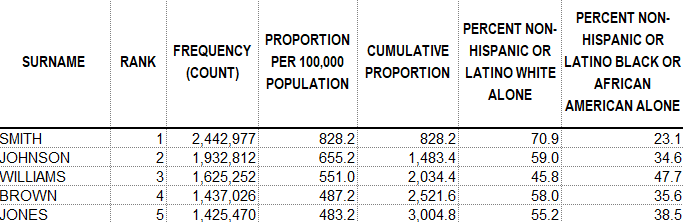
\includegraphics{census.png}}}}
\end{frame}
}

\frame{

\Large{But if were to learn from names, how would we?}
\begin{large_enum}
	\item[-]<0>$p\;(\text{ethnicity\;}|\;\text{name})$?
	\item[-]<0> Classify to the majority class
	\item[-]<0> Makes the least mistakes if that is all you have
	\item[-]<0-> Census Last Name Dataset
		\begin{itemize}
			\item[-]<1->Split by race for \alert<2>{1,000} most common last names
		\end{itemize}
\end{large_enum}
}

\frame{

\Large{\only<1>{Problems}\only<2>{\sout{\alert{Problems}}}\only<3->{Opportunities}}
\begin{large_enum}
  \item[-]<4> Classifying the other 160k+ last names
  \item[-]<5-6> When we have more than the last name\\
  \only<6->{\normalsize{e.g., African-Americans have more distinctive first names}}
  \item[-]<7> When we have minor variations
  \item[-]<8> Geographic variation
\end{large_enum}
}

\frame{
\only<1->{\Large{How to capitalize on the opportunities?}}
\begin{large_enum}
  \item[-]<2> Patterns in names
  \item[-]<3> Capturing sounds, sequence of sounds, \ldots
  \item[-]<4-6> Phonemes are dead. Long live bi-chars! \\
  \only<5->{\normalsize{\texttt{da\_as\_sh\_ia\_an,}} \only<6->{\texttt{jo\_oh\_ha\_an\_ns\_so\_on}}}
  \item[-]<7> Patterns in communication networks, e.g., Skiena et al. 2018.
\end{large_enum}
}

\frame{
\Large{How to Classify Text\\}

\begin{large_enum}
   \item[-]<1-5> Text $\leadsto$ Embeddings $\leadsto$ Classifier
		\begin{enumerate}
			\item[-]<2-> Embeddings leverage the adage:\\
						  You are the company you keep.
			\item[-]<3-> Use a large corpus
			\item[-]<4-> Learn the context well
			\item[-]<5-> Preserve tens of hundreds of vectors and pass them to a model 
	    \end{enumerate}
	
	\item[-]<6->In Our Case:
		\begin{enumerate}
			\item[-]<7-> Embeddings of common bi-chars
			\item[-]<8-> LSTM
		\end{enumerate}
	\end{large_enum}
}

\frame{

\Large{But what do you mean by race and ethnicity? \vspace{5mm}}
\begin{large_enum}
	\item[-]<2-3> How would I describe myself?\\
				\only<3->{\normalsize{Indian? But there is systematic variation across names across linguistic groups within India.}}
	\item[-]<4> Are you willing to fight for the \texttt{group}?
	\item[-]<5> How people describe themselves in free text?
	\item[-]<6> What do people choose when asked to force-fit into administrative categories?
\end{large_enum}
}

\frame{
\Large{Data}
\begin{large_enum}
		 \item[-]<2-> Voting Registration data from Florida\\

		 \item[-]<3-> Race/Ethnicity = Asian or Pacific Islander, Hispanic, NH Black, NH White
		 \item[-]<4-> Wikipedia $\sim$ Famous people but more finely coded race
	\end{large_enum}
}

\frame{
\Large{Success Using Florida Voter Registration Data}
\only<2->{
		\begin{table}[!htb] 
		\small
		\centering
		\begin{tabular}{|cc|cc|}
			\hline
			   			& 		 & \multicolumn{2}{c|}{\textbf{F1-Score}} \\
			   			& 		 & Last Name 			& Full Name\\[0.5ex]
				\cline{2-4}
				\textbf{Race}    & Asian      &   .54     & .60\\[0.5ex]
				        	     & Hispanic   &   .72     & .75\\[0.5ex]
				        	     & \alert<2-3>{NH Black}   &   \alert<2-3>{.32}     & \alert<3>{.55}\\[0.5ex]
				        	     & NH White   &   .88     & .90\\[0.5ex]
			    \hline
		\end{tabular}
		\end{table}
		}
}

\frame{
\Large{\only<1>{Donations to Political Campaigns in 2000 and 2010 by Race and Ethnicity}}
\only<2->{
\begin{table}[h!]
\centering
\begin{tabular}{ l c c c c}
\hline
         & \multicolumn{2}{c}{Census} & \multicolumn{2}{c}{Florida}\\
\hline
     &     2000     & 2010     &    2000    & 2010\\    
\hline
asian    &     2.2\%   & 2.7\%   &   2.0\%   & 2.3\%\\
black    &     11.0\%  & 10.2\%  &   8.9\%   & 7.9\%\\
hispanic &     \alert<2-3>{3.2\%}   & \alert<2-3>{4.3\%}   &   \alert<2-3>{3.2\%}   & \alert<2-3>{3.3\%}\\
white    &     83.5\%  & 82.7\%  &   85.8\%  & \alert<3>{86.5\%}\\
\hline
\end{tabular}
\label{table:percentage_contrib_by_race}
\end{table}
}
}

\frame{
	\frametitle{Python Package}
\begin{lstlisting}
# pip install ethnicolr

> import pandas as pd

> from ethnicolr import census\_ln, pred\_census\_ln \\
Using TensorFlow backend.

> names = [{`name': `smith'}, \\
...         {`name': `zhang'}, \\
...         {`name': `jackson'}] \\

> df = pd.DataFrame(names)

> census\_ln(df, `name', 2010) \\
\end{lstlisting}

\begin{table}[h!]
\centering
\begin{tabular}{ l llll}
name     &   race   & pctwhite &  pctblack & pctapi\\    
smith    &   white  &  70.9    &  23.11    & 0.5\\
zhang    &   api 	& 0.99     &  0.16     & 98.06\\
jackson  &   black 	& 39.89    &  53.04    & 0.39\\
\end{tabular}
\label{table:percentage_contrib_by_race}
\end{table}
}


\end{document}
